% \documentclass[acmtog,review,anonymous]{acmart}
\documentclass[acmtog,nonacm]{acmart}

%%
%% \BibTeX command to typeset BibTeX logo in the docs
\AtBeginDocument{%
  \providecommand\BibTeX{{%
    \normalfont B\kern-0.5em{\scshape i\kern-0.25em b}\kern-0.8em\TeX}}}

%% Rights management information.  This information is sent to you
%% when you complete the rights form.  These commands have SAMPLE
%% values in them; it is your responsibility as an author to replace
%% the commands and values with those provided to you when you
%% complete the rights form.
% \acmJournal{TOG}
% \setcopyright{acmlicensed}
% \copyrightyear{2024}
% \acmYear{2024}
\acmYear{2025} 
% \acmVolume{0} 
% \acmNumber{0} 
% \acmArticle{0}
% \acmMonth{0}
% \acmDOI{}


\usepackage{enumitem}
\usepackage{graphicx}
\usepackage{subcaption}
\usepackage{booktabs}
\usepackage{multirow}
\usepackage{xspace}

\newcommand{\ly}[1]{{\color{magenta} {[Yuan: #1]}}}
\newcommand{\ZY}[1]{{\color{blue} {[#1]}}}

\newcommand{\methodname}{DaS\xspace}

%% These commands are for a PROCEEDINGS abstract or paper.
% \acmConference[Conference acronym 'XX]{Make sure to enter the correct
%   conference title from your rights confirmation emai}{June 03--05,
%   2018}{Woodstock, NY}
%
%  Uncomment \acmBooktitle if th title of the proceedings is different
%  from ``Proceedings of ...''!
%
%\acmBooktitle{Woodstock '18: ACM Symposium on Neural Gaze Detection,
%  June 03--05, 2018, Woodstock, NY} 
% \acmISBN{978-1-4503-XXXX-X/18/06}
% \acmSubmissionID{papers\_xxx}
\citestyle{acmauthoryear}

\begin{document}

\title{Diffusion as Shader: 3D-aware Video Diffusion for Versatile Video Generation Control}


% \begin{CCSXML}
% <ccs2012>
%     <concept>
%         <concept_id>10010147.10010371.10010372</concept_id>
%         <concept_desc>Computing methodologies~Rendering</concept_desc>
%         <concept_significance>500</concept_significance>
%     </concept>
% </ccs2012>
% \end{CCSXML}

% \ccsdesc[500]{Computing methodologies~Rendering}



\author{Zekai Gu}
\affiliation{
  \institution{Hong Kong University of Science and Technology}
  \city{Hong Kong}
  \country{China}
}
\author{Rui Yan}
\affiliation{
  \institution{Zhejiang University}
  \city{Hangzhou}
  \country{China}
}
\author{Jiahao Lu}
\affiliation{
  \institution{Hong Kong University of Science and Technology}
  \city{Hong Kong}
  \country{China}
}
\author{Peng Li}
\affiliation{
  \institution{Hong Kong University of Science and Technology}
  \city{Hong Kong}
  \country{China}
}
\author{Zhiyang Dou}
\affiliation{
  \institution{The University of Hong Kong}
  \city{Hong Kong}
  \country{China}
}
\author{Chenyang Si}
\affiliation{
  \institution{Nanyang Technological University}
  \city{Singapore}
  \country{Singapore}
}
\author{Zhen Dong}
\affiliation{
  \institution{Wuhan University}
  \city{Wuhan}
  \country{China}
}
\author{Qifeng Liu}
\affiliation{
  \institution{Hong Kong University of Science and Technology}
  \city{Hong Kong}
  \country{China}
}
\author{Cheng Lin}
\affiliation{
  \institution{The University of Hong Kong}
  \city{Hong Kong}
  \country{China}
}
\author{Ziwei Liu}
\affiliation{
  \institution{Nanyang Technological University}
  \city{Singapore}
  \country{Singapore}
}
\author{Wenping Wang}
\affiliation{%
  \institution{Texas A\&M University}
  \city{Texas}
  \country{U.S.A}
}
\author{Yuan Liu}
\affiliation{
  \institution{Hong Kong University of Science and Technology}
  \city{Hong Kong}
  \country{China}
}
\makeatletter
\let\@authorsaddresses\@empty
\makeatother
\renewcommand{\shortauthors}{Zekai Gu, et al.}

\begin{abstract}
We introduce Causal Diffusion as the autoregressive (AR) counterpart of Diffusion models. It is a next-token(s) forecasting framework that is friendly to both discrete and continuous modalities and compatible with existing next-token prediction models like LLaMA and GPT. While recent works attempt to combine diffusion with AR models, we show that introducing sequential factorization to a diffusion model can substantially improve its performance and enables a smooth transition between AR and diffusion generation modes. Hence, we propose \textbf{CausalFusion} - a decoder-only transformer that dual-factorizes data across sequential tokens and diffusion noise levels, leading to state-of-the-art results on the ImageNet generation benchmark while also enjoying the AR advantage of generating an arbitrary number of tokens for in-context reasoning. We further demonstrate CausalFusion's multimodal capabilities through a joint image generation and captioning model, and showcase CausalFusion's ability for zero-shot in-context image manipulations. We hope that this work could provide the community with a fresh perspective on training multimodal models over discrete and continuous data.
\end{abstract}
\vspace{-10pt}
\section{Introduction}
\label{sec:intro}
Autoregressive (AR) and diffusion models are two powerful paradigms for data distribution modeling. AR models, also known as the next token prediction approach, dominate language modeling and are considered central to the success of large language models (LLMs)~\cite{gpt1,gpt2,gpt3,llama1,llama2,llama3}. On the other hand, diffusion models~\cite{ddpm,dit,adm,edm}, or score-based generative models~\cite{songscore,lipman2023flow}, have emerged as the leading approach for visual generation, driving unprecedented progress in the era of visual content generation~\cite{sora,rombach2022high,li2023scaling}. 

\begin{figure}[t]
    \centering
    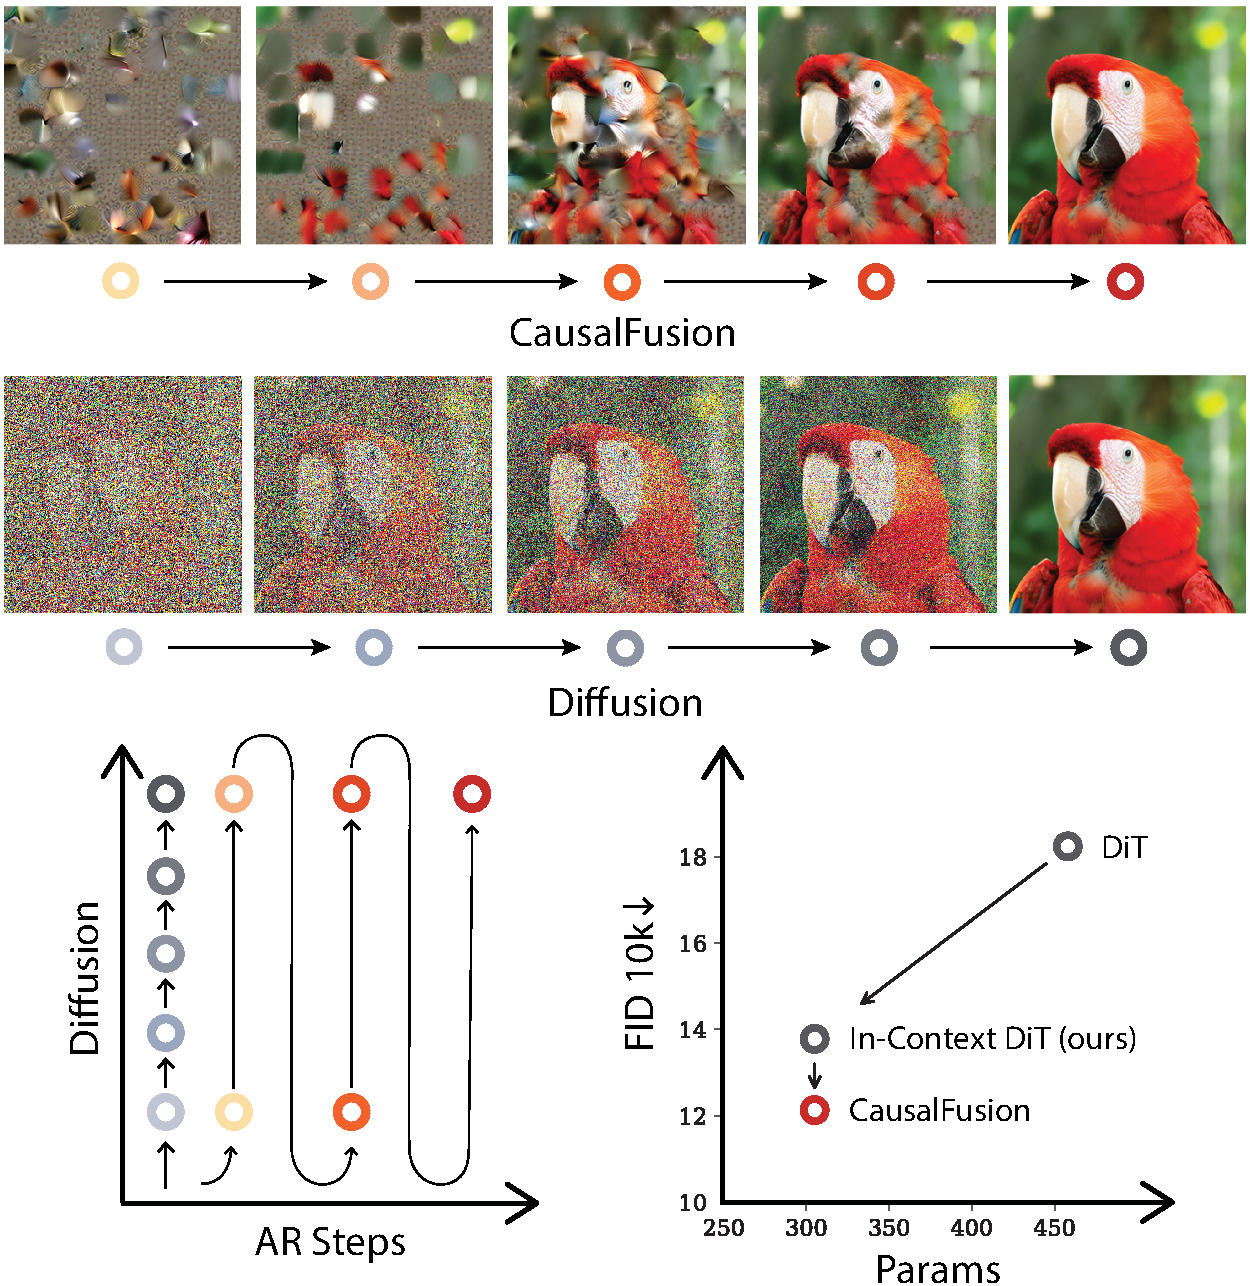
\includegraphics[width=1.0\textwidth,height=1.0\textwidth]{figs/casualfusion-teaser-v6.pdf} 
    \vspace*{-6mm}
    \caption{
    \textbf{Illustration of Dual-Factorization}. The arrow line indicates CausalFusion's generation path, moving from one state to the next by jointly generating along the sequential and noise-level dimension at each step. 
    Compared to DiT, our In-context DiT substantially improves results with fewer parameters. CausalFusion further enhances performance without changing the architecture or parameter count. Results were trained on IN1K for 240 epochs. CausalFusion adopts arbitrary AR steps for image generation, but each step only diffuses partial tokens, resulting in similar (or slightly lower) computational complexity.
    \vspace{-10pt}
    }
    \label{fig:dual-factorization}
\end{figure}


\begin{figure*}[t]
  \centering
  \begin{subfigure}{1.0\linewidth}
    \centering
    \includegraphics[width=\linewidth]{figs/figure2.pdf}
    \caption{Samples generated by CausalFusion-XL/2, ImageNet 512$\times$512, 800 epoch, DDPM 250 steps, CFG=4.0}
  \end{subfigure}
  \begin{subfigure}{1.0\linewidth}
    \centering
    \includegraphics[width=\linewidth]{figs/edit.pdf}
    \caption{\textbf{Zero-shot image editing} results generated by CausalFusion-XL/2, ImageNet 512$\times$512, 800 epoch. We first generate the original image (those on the left), then mask out its centre region, top-half, or bottom-half, and regenerate the image with new class conditions. Details are discussed in Sec \ref{sec:system}.}
  \end{subfigure}
  \caption{\textbf{Visualization results}. All samples are generated by models trained only on \textbf{ImageNet-1K class-conditional generation} task, demonstrating CausalFusion's zero-shot image manipulation ability. See more visualization results in Appendix~\ref{appendix:secD}.
  \vspace{-12pt}
  }
  \vspace{-6pt}
  \label{fig:vis1}
\end{figure*}

The intrinsic distinction between AR and diffusion models lies in their approach to data distribution factorization. AR models treat data as an ordered sequence, factorizing it along the sequential axis, where the probability of each token is conditioned on all preceding tokens. This factorization enables the AR paradigm to generalize effectively and efficiently across arbitrary number of tokens, making it well-suited for long-sequence reasoning and in-context generation. In contrast, diffusion models factorize data along the noise-level axis, where the tokens at each step are a refined (denoised) version of themselves from the previous step. As a result, the diffusion paradigm is generalizable to arbitrary number of data refinement steps, enabling iterative quality improvement with scaled inference compute. While AR and diffusion models each excel within their respective domains, their distinct factorization approaches reveal complementary potential. Although recent studies~\cite{transfusion,monoformer,dart} have attempted to integrate AR and diffusion within a single model, they typically treat these paradigms as separate modes, missing the potential benefits of jointly exploring them within a 2-D factorization plane.

To this end, we introduce \textbf{CausalFusion}, a flexible framework that integrates both sequential and noise-level data factorization to unify their advantages. The degree of factorization along these two axes—namely, the AR step and diffusion step—is adjustable, enabling {CausalFusion} to revert seamlessly to the traditional AR or diffusion paradigms at either extreme. To enhance its generality, CausalFusion is designed to predict \textit{any} number of tokens at \textit{any} AR step, with \textit{any} pre-defined sequence order and \textit{any} level of inference compute, thereby minimizing the inductive biases presented in existing generative models. As shown in Figure~\ref{fig:dual-factorization}, this approach provides a broad spectrum between the AR and diffusion paradigms, allowing smooth interpolation within two endpoints during both training and inference. 
Specifically, we explore CausalFusion in image generation and multimodal generation scenarios, where we observe that the level of training difficulties significantly influences the overall effectiveness of CausalFusion.

\textbf{Difficulties of generative tasks in CausalFusion:} Both AR and diffusion paradigms present unique challenges based on difficulties of their specific generative stages. In diffusion models, the effectiveness of training depends heavily on proper loss weighting across noise levels~\cite{ddpm,minsnr}, as higher noise levels are more difficult and usually provide more valuable signals than lower noise levels. Similarly, AR models are susceptible to error accumulation~\cite{bengio2015scheduled} as early-stage predictions are made with limited visible context, making them more error-prone. Optimizing CausalFusion thus requires balancing across these varying task difficulties to optimize training signal impact and ensure sufficient exploration across the entire factorization plane.

In this paper, we formally examine the difficulties of generative tasks within CausalFusion. We show that, in addition to the noise levels in diffusion and the amount of visible context in AR, the total number of AR steps, which controls the interpolation between AR and diffusion, also plays a critical role in shaping training difficulties. Driven by these factors, we develop a scalable and versatile model based on the CausalFusion framework. Starting from the DiT architecture~\cite{dit}, we gradually convert it into a decoder-only transformer compatible with existing AR models like GPT~\cite{gpt1,gpt2,gpt3} and LLaMA~\cite{llama1,llama2,llama3}. We provide insights on how to appropriately choose the number of AR steps during the training of CausalFusion models, and further introduce loss weighing along both the diffusion and AR axis to balance the impact of different generative stages. As shown in Figure~\ref{fig:dual-factorization} and ~\ref{fig:vis1}, our model achieves state-of-the-art performance on the ImageNet class-conditional generation benchmark, significantly outperforming DiT~\cite{dit} and enabling zero-shot image manipulations due to its AR nature. When pretraining on both text-to-image and image-to-text tasks, our model surpasses forced-fusion frameworks such as TransFusion~\cite{transfusion}, demonstrating the versatility of our CausalFusion framework.


We highlight our main contribution below:
\begin{itemize}
\item  We propose CausalFusion as the AR counterpart to DiT, achieving state-of-the-art results and enabling the unlimited token generation for in-context reasoning.
\item  We systematically study CausalFusion on the dual-factorization plane and identify key factors that improve the effectiveness of CausalFusion models.
\item  Compared with recent studies~\cite{transfusion}, CausalFusion enables a smooth, cohesive integration with language modeling for cross-modal generation and reasoning.
\end{itemize} 

% \begin{figure}[t]
%   \begin{minipage}{0.49\textwidth}
%      \centering
%     \includegraphics[width=1.0\textwidth]{fig/MLMF.png}
%     \caption{Multi-Layer Motion Fusion.}
%     \label{fig: frameselector_abalation}
    
%   \end{minipage}
%   \hfill
%    \begin{minipage}{0.48\textwidth}
%     \centering
%     \includegraphics[width=0.8\textwidth]{fig/SMPL.jpg}
%     \caption{Prametric Shape Alignment.}
%     \label{fig:Visualizedselected_frames}
%   \end{minipage}
% \vspace{-3mm}
% \end{figure}


\section{Related Work}
\label{sec:related_work}

\textbf{Diffusion Models for Image Generation.}
Diffusion-based models~\cite{balaji2022ediffi,huang2023composer,nichol2021glide,ramesh2022hierarchical,rombach2022high,saharia2022photorealistic} have rapidly emerged as a fundamental component in the domain of text-to-image generation, renowned for their capacity to yield highly promising generative outcomes. 
To address the considerable computational requirements inherent in diffusion models, the Latent Diffusion Model, as proposed in~\cite{rombach2022high} introduces a technique for denoising within the latent space.
This method not only enhances the computational efficiency of these models but also preserves their ability to generate high-fidelity images.
Moreover, in the endeavor to enhance control over visual generation, recent studies such as ControlNet~\cite{zhang2023adding}, T2I-Adapter~\cite{mou2023t2i}, and IP-Adapter~\cite{ye2023ip} have delved into the incorporation of supplementary encoder layers.
These layers facilitate the assimilation of control signals encompassing aspects such as pose, depth, and edge information, and even permit the utilization of images in conjunction with textual prompts.
This progression signifies a significant advancement towards more controlled and precise image generation, facilitating the creation of images characterized by not only superior quality but also enriched contextual accuracy and detail.


\textbf{Diffusion Models for Human Image Animation.}
The task of animating human images, a significant endeavor within the domain of video generation, aims to seamlessly create videos from one or multiple static images~\cite{chan2019everybody,ren2020deep,siarohin2019first,siarohin2021motion,yu2023bidirectionally,zhang2022exploring,zhao2022thin,yoon2021pose, sarkar2021neural, hu2023sherf, albahar2023humansgd, cao2023dreamavatar, prokudin2021smplpix, fu2022styleganhuman, jiang2023humangen}.
The recent advancements of diffusion models in the text-to-image domain have sparked interest in exploring their utility for animating human images.
PIDM~\cite{bhunia2023person} introduces a texture diffusion module that is specifically crafted to align the texture patterns of the source and target images closely, thereby enhancing the realism of the resultant animated output.
DreamPose~\cite{karras2023dreampose} capitalizes on the capabilities of the pre-trained Stable Diffusion model by incorporating both CLIP~\cite{radford2021learning} and VAE~\cite{kingma2013auto} for image encoding. 
It integrates these embeddings with an adapter. 
Similarly, DisCo~\cite{wang2023disco} innovatively segregates the control of pose and background using dual independent ControlNets~\cite{zhang2023adding}, providing finer control over the animation process. 
Animate Anyone~\cite{hu2023animate} utilizes a UNet-based ReferenceNet to extract features from reference images.
It includes pose information via a lightweight pose guider. Expanding on the principles introduced by AnimateDiff~\cite{guo2023animatediff}, Animate Anyone integrates a temporal layer into the denoising UNet to enhance temporal coherence.
MagicAnimate~\cite{xu2023magicanimate} follows a similar approach but employs a ControlNet tailored for DensePose \cite{guler2018dense} inputs instead of the more commonly used OpenPose~\cite{cao2017realtime} keypoints to provide more precise pose guidance.
This paper primarily builds upon esteemed diffusion-based methodologies and advances the optimization of appearance alignment and motion guidance mechanisms. 
This is achieved by introducing a 3D parametric model for geometric reconstruction of the reference image and motion modeling of the source video sequence.


\textbf{Pose Guidance in Human Image Animation.}
DWpose\cite{yang2023effective} stands out as an enhanced alternative to OpenPose\cite{cao2017realtime}, offering more accurate and expressive skeletons. 
This improvement has proven beneficial for diffusion models in generating higher quality images, with its adoption as a condition signal in various works\cite{feng2023dreamoving,hu2023animate}.
The work presented in DensePose~\cite{Guler2018DensePose} aims to establish dense correspondences between an RGB image and a surface-based representation.
The SMPL~\cite{SMPL:2015} model is a 3D model renowned for its realistic depiction of human bodies through skinning and blend shapes.
Its widespread adoption spans fields like human reconstruction\cite{he2021arch,alldieck2018video} and interaction with environments\cite{hassan2021populating,ma2020learning}. 
It also serves as essential ground truth for neural networks in pose and shape analysis\cite{lu2023dposer,mu2023actorsnerf}.
In this paper, we consider SMPL, the 3D parametric model, to reconstruct the poses as well as the shapes from the source video, and obtain more complete condition for appearance alignment and pose guidance.

\begin{figure}[t]
  \centering
  \includegraphics[width=0.95\linewidth]{fig/framework.jpg}
  \caption{The overview of our proposed approach. Given an input human image and a reference video depicting a motion sequence. We obtain the pose sequence corresponding to the reference image through Parametric Shape Alignment as 3D motion guidance. MLMF is employed to encode multi-layer 3D-related motion information. Referencenet and Temporal-attention ensure identity consistency and temporal coherence, respectively.}
  \vspace{-6mm}
  \label{fig:network}
\end{figure}
\section{Method}
%%%%%%%%% Figure: Overall framework
\begin{figure*}[t]
  \centering
   \includegraphics[width=0.85\linewidth]{figures/PoolFormer_overall_architecture.pdf}
   \vspace{-4mm}
   \caption{\textbf{(a) The overall framework of \modelname{}.} Similar to \cite{resnet, pvt, swin}, \modelname{} adopts hierarchical architecture with 4 stages. For a model with L \modelname{} blocks, stage [1, 2, 3, 4] have [L/6, L/6, L/2, L/6] blocks, respectively. The feature dimension $D_i$ of stage $i$ is shown in the figure. \textbf{(b) The architecture of \modelname{} block.} Compared with Transformer block, it replaces attention with extremely simple non-parametric operator, pooling, to conduct only basic token mixing.}
   \label{fig:overall_architecture}
\end{figure*}


%%%%%%%%% Algorithm: Pooling
\begin{algorithm}[t]
\caption{Pooling for PoolFormer, PyTorch-like Code}
\label{alg:code}
\definecolor{codeblue}{rgb}{0.25,0.5,0.5}
\definecolor{codekw}{rgb}{0.85, 0.18, 0.50}
\lstset{
  backgroundcolor=\color{white},
  basicstyle=\fontsize{7.5pt}{7.5pt}\ttfamily\selectfont,
  columns=fullflexible,
  breaklines=true,
  captionpos=b,
  commentstyle=\fontsize{7.5pt}{7.5pt}\color{codeblue},
  keywordstyle=\fontsize{7.5pt}{7.5pt}\color{codekw},
}
\begin{lstlisting}[language=python]
import torch.nn as nn

class Pooling(nn.Module):
    def __init__(self, pool_size=3):
        super().__init__()
        self.pool = nn.AvgPool2d(
            pool_size, stride=1, 
            padding=pool_size//2, 
            count_include_pad=False,
        )
    def forward(self, x):
        """
        [B, C, H, W] = x.shape
        Subtraction of the input itself is added 
        since the block already has a 
        residual connection.
        """
        return self.pool(x) - x
\end{lstlisting}
\end{algorithm}

\subsection{MetaFormer}
We present the core concept ``MetaFormer" for this work at first. As shown in Figure \ref{fig:first_figure}, abstracted from Transformers \cite{transformer}, 
MetaFormer is a general architecture where the token mixer is not specified while the other components are kept the same as Transformers. The input $I$ is first processed by input embedding, such as  patch embedding for ViTs \cite{vit},
\begin{equation}
    X = \mathrm{InputEmb}(I),
\end{equation}
where  $X \in \mathbb{R}^{N \times C}$ denotes the embedding tokens with sequence length $N$ and embedding dimension $C$. 


Then, embedding tokens are fed to repeated MetaFormer blocks, each of which includes two residual sub-blocks. Specifically, the first sub-block mainly contains a token mixer to communicate information among tokens and this sub-block can be expressed as
\begin{equation}
    Y = \mathrm{TokenMixer}(\mathrm{Norm}(X)) + X,
\end{equation}
where $\mathrm{Norm}(\cdot)$ denotes the normalization such as Layer Normalization \cite{layer_norm} or Batch Normalization \cite{batch_norm}; $\mathrm{TokenMixer}(\cdot)$ means a module mainly working for mixing token information. It is implemented by various attention mechanism in recent vision Transformer models  \cite{vit,refiner,t2t} or spatial MLP in MLP-like models \cite{mlp-mixer, resmlp}. Note that the main function of the token mixer is to propagate token information although some token mixers can also mix channels, like attention. 


The second sub-block primarily consists of a two-layered MLP with non-linear activation, 
\begin{equation}
    Z = \sigma(\mathrm{Norm}(Y)W_1)W_2 + Y,
\end{equation}
where $W_1 \in \mathbb{R}^{C \times rC}$ and $W_2 \in \mathbb{R}^{rC \times C}$ are learnable parameters with MLP expansion ratio $r$; $\sigma(\cdot)$ is a non-linear activation function, such as GELU \cite{gelu} or ReLU \cite{relu}. 

\myPara{Instantiations of MetaFormer} MetaFormer describes a general architecture 
% a general architecture that is powerful at solving computer vision tasks.  
with which different models can be obtained immediately by specifying the concrete design of the token mixers. 
As shown in Figure \ref{fig:first_figure}(a), if the token mixer is specified as attention or spatial MLP, MetaFormer then becomes a Transformer or MLP-like model respectively. 

\subsection{PoolFormer}
From the introduction of Transformers \cite{transformer}, lots of works attach much importance to the attention and focus on designing various attention-based token mixer components. In contrast, these works pay little attention to the general architecture, \ie, the MetaFormer.


In this work, we argue that this MetaFormer general architecture contributes mostly to the success of the recent Transformer and MLP-like models. 
To demonstrate it, we deliberately employ an embarrassingly simple operator, pooling, as the token mixer. This operator has no learnable parameters and it just makes each token averagely aggregate its nearby token features. 


Since this work is targeted at vision tasks,  we assume the input is in channel-first data format, \ie,  $T \in \mathbb{R}^{C \times H \times W}$. The pooling operator can be expressed as
\begin{equation}
\label{eq:pool}
    T'_{:, i, j} =  \frac{1}{K \times K} \sum_{p,q=1}^{K}T_{:, i+p-\frac{K+1}{2}, i+q-\frac{K+1}{2}} - T_{:, i, j},
\end{equation}
where $K$ is the pooling size. Since the MetaFormer block already has a residual connection, subtraction of the input itself is added in Equation (\ref{eq:pool}). The PyTorch-like code of the pooling is shown in Algorithm \ref{alg:code}.


As well known, self-attention and spatial MLP have computational complexity quadratic to the number of tokens to mix. Even worse, spatial MLPs bring much more parameters when handling longer sequences. As a result, self-attention and spatial MLPs usually can only process hundreds of tokens. In contrast, the pooling needs a computational complexity linear to the sequence length without any learnable parameters.  Thus, we take advantage of pooling by adopting a hierarchical structure similar to traditional CNNs \cite{alexnet, vgg, resnet} and recent hierarchical Transformer variants \cite{swin, pvt}. Figure \ref{fig:overall_architecture} shows the overall framework of PoolFormer. Specifically, PoolFormer has 4 stages with $\frac{H}{4} \times \frac{W}{4}$, $\frac{H}{8} \times \frac{W}{8}$, $\frac{H}{16} \times \frac{W}{16}$, and $\frac{H}{32} \times \frac{W}{32}$ tokens respectively, where $H$ and $W$ represent the width and height of the input image. There are two groups of embedding size: 1) small-sized models with embedding dimensions of 64, 128, 320, and 512 responding to the four stages; 2) medium-sized models with embedding dimensions 96, 192, 384, and 768. Assuming there are $L$ PoolFormer blocks in total, stages 1, 2, 3, and 4 will contain $L/6$, $L/6$, $L/2$, and $L/6$ PoolFormer blocks respectively. The MLP expansion ratio is set as 4. According to the above simple model scaling rule, we obtain 5 different model sizes of PoolFormer and their hyper-parameters are shown in Table \ref{tab:model}.


%%%%%%%%% Table: Model Configurations
\begin{table}[t]
\footnotesize
\centering
\setlength{\tabcolsep}{2pt}
% \scalebox{0.65}{\newcommand{\blockc}[4]{
$\begin{bmatrix}
	\begin{array}{l}
	R_1=#1 \\
	N_1=#2 \\
	E_1=#3 \\
	\end{array}
\end{bmatrix} \times #4$
}

\newcommand{\sblock}[3]{
$\begin{matrix}
E_{#1}=#2 \\
L_{#1}=#3 \\
\end{matrix}$
}

\newcommand{\poollayer}{
Pooling Size & \multicolumn{5}{c}{$3 \times 3$, stride 1}\\
\cline{4-9}
}

\newcommand{\stitle}[6]{
\multirow{5}{*}{#1} & \multirow{5}{*}{\scalebox{1}{$\frac{H}{#2}\times \frac{W}{#2}$}} & \multirow{2}{*}{\tabincell{c}{Patch \\ Embedding}} & Patch Size & \multicolumn{5}{c}{$#3 \times #3$, stride $#4$} \\
\cline{4-9}
    &    &    & Embed. Dim. & \multicolumn{3}{c|}{$#5$} & \multicolumn{2}{c}{$#6$} \\
\cline{3-9}
& & \multirow{3}{*}{\tabincell{c}{\modelname{}\\Block}} 
}

\begingroup
\renewcommand{\arraystretch}{1.1}
\begin{tabular}{c|c|c|c|c|c|c|c|c}
\toprule
  \multirow{2}{*}{Stage} & \multirow{2}{*}{\#Tokens} & \multicolumn{2}{c|}{\multirow{2}{*}{Layer Specification}} & \multicolumn{5}{c}{\modelname{}} \\
\cline{5-9}
 & & \multicolumn{2}{c|}{} & S12 & S24 & S36 & M36 & M48 \\
\whline
\stitle{1}{4}{7}{4}{64}{96}    & \poollayer
 & & & MLP Ratio & \multicolumn{5}{c}{4} \\
\cline{4-9}
 & & & \# Block & 2 & 4 & 6 & 6 & 8 \\
\hline
\stitle{2}{8}{3}{2}{128}{192}  & \poollayer
 & & & MLP Ratio & \multicolumn{5}{c}{4} \\
 \cline{4-9}
 & & & \# Block & 2 & 4 & 6 & 6 & 8 \\
\hline
\stitle{3}{16}{3}{2}{320}{384} & \poollayer
 & & & MLP Ratio & \multicolumn{5}{c}{4} \\
\cline{4-9}
 & & & \# Block & 6 & 12 & 18 & 18 & 24 \\
\hline
\stitle{4}{32}{3}{2}{512}{768} & \poollayer
 & & & MLP Ratio & \multicolumn{5}{c}{4} \\
 \cline{4-9}
 & & & \# Block & 2 & 4 & 6 & 6 & 8 \\
\hline
\multicolumn{4}{c|}{Parameters~(M)}& 11.9 & 21.4              &  30.8            &  56.1              &  73.4    \\
\hline
\multicolumn{4}{c|}{MACs~(G)}     & 1.8  &  3.4              &  5.0             &  8.8              &  11.6    \\
\bottomrule
\end{tabular}
\endgroup
}
\newcommand{\blockc}[4]{
$\begin{bmatrix}
	\begin{array}{l}
	R_1=#1 \\
	N_1=#2 \\
	E_1=#3 \\
	\end{array}
\end{bmatrix} \times #4$
}

\newcommand{\sblock}[3]{
$\begin{matrix}
E_{#1}=#2 \\
L_{#1}=#3 \\
\end{matrix}$
}

\newcommand{\poollayer}{
Pooling Size & \multicolumn{5}{c}{$3 \times 3$, stride 1}\\
\cline{4-9}
}

\newcommand{\stitle}[6]{
\multirow{5}{*}{#1} & \multirow{5}{*}{\scalebox{1}{$\frac{H}{#2}\times \frac{W}{#2}$}} & \multirow{2}{*}{\tabincell{c}{Patch \\ Embedding}} & Patch Size & \multicolumn{5}{c}{$#3 \times #3$, stride $#4$} \\
\cline{4-9}
    &    &    & Embed. Dim. & \multicolumn{3}{c|}{$#5$} & \multicolumn{2}{c}{$#6$} \\
\cline{3-9}
& & \multirow{3}{*}{\tabincell{c}{\modelname{}\\Block}} 
}

\begingroup
\renewcommand{\arraystretch}{1.1}
\begin{tabular}{c|c|c|c|c|c|c|c|c}
\toprule
  \multirow{2}{*}{Stage} & \multirow{2}{*}{\#Tokens} & \multicolumn{2}{c|}{\multirow{2}{*}{Layer Specification}} & \multicolumn{5}{c}{\modelname{}} \\
\cline{5-9}
 & & \multicolumn{2}{c|}{} & S12 & S24 & S36 & M36 & M48 \\
\whline
\stitle{1}{4}{7}{4}{64}{96}    & \poollayer
 & & & MLP Ratio & \multicolumn{5}{c}{4} \\
\cline{4-9}
 & & & \# Block & 2 & 4 & 6 & 6 & 8 \\
\hline
\stitle{2}{8}{3}{2}{128}{192}  & \poollayer
 & & & MLP Ratio & \multicolumn{5}{c}{4} \\
 \cline{4-9}
 & & & \# Block & 2 & 4 & 6 & 6 & 8 \\
\hline
\stitle{3}{16}{3}{2}{320}{384} & \poollayer
 & & & MLP Ratio & \multicolumn{5}{c}{4} \\
\cline{4-9}
 & & & \# Block & 6 & 12 & 18 & 18 & 24 \\
\hline
\stitle{4}{32}{3}{2}{512}{768} & \poollayer
 & & & MLP Ratio & \multicolumn{5}{c}{4} \\
 \cline{4-9}
 & & & \# Block & 2 & 4 & 6 & 6 & 8 \\
\hline
\multicolumn{4}{c|}{Parameters~(M)}& 11.9 & 21.4              &  30.8            &  56.1              &  73.4    \\
\hline
\multicolumn{4}{c|}{MACs~(G)}     & 1.8  &  3.4              &  5.0             &  8.8              &  11.6    \\
\bottomrule
\end{tabular}
\endgroup

\vspace{-3mm}
\caption{\textbf{ Configurations of different PoolFormer models.} There are two groups of embedding dimensions, \ie, small size with [64, 128, 320, 512] dimensions and medium size with [96, 196, 384, 768]. Notation ``S24" means the model is in small size of embedding dimensions with 24 PoolFormer blocks in total. The numbers of MACs are counted by \texttt{fvcore}\cite{fvcore} library.
}
\label{tab:model}
\vspace{-4mm}
\end{table}

\begin{figure*}[htbp]
    \centering
    \includegraphics[width=1.0\linewidth]{figs/exp-applications.pdf}
    \vspace{-0.2in}
    \caption{\textbf{Applications.} \textbf{Top}: Text-to-Video with Transparency. \textbf{Bottom}: Image-to-Video generation with transparency.
.}
    \label{fig-applications}
    \vspace{-0.1in}
\end{figure*}


\section{Experiment}
\label{sec:exp}

%-------------------------------------------------------------------------
%\subsection{Implementation Details}

\noindent\textbf{Training Dataset.}~We utilize the public VideoMatte240K dataset~\cite{lin2021real}, a comprehensive collection of 484 high-resolution green screen videos consists of 240,709 unique frames of alpha mattes and foregrounds. These frames provide a diverse range of human subjects, clothing styles, and poses. We apply fundamental preprocessing steps for them, including color decontamination and background blurring. Prompts are extracted using ShareGPT4V~\cite{chen2023sharegpt4v}. 

\vspace{0.5em}
\noindent\textbf{Model.}~Our RGBA video diffusion models are developed by fine-tuning pre-trained diffusion models. Specifically, we employ two models based on the diffusion transformer architecture: the open-source model CogVideoX~\cite{yang2024cogvideox} and a modified variant of CogVideoX denoted as \(J\). 
CogVideoX generates RGB videos at a resolution of 480x720 with 49 frames at 8 FPS, using 50 sampling steps. In contrast, the modified version produces videos at a resolution of 176x320 with 64 frames at 24 FPS, while also using 50 sampling steps. Additionally, we integrate our method with CogVideoX-I2V (Image-to-Video) to support image-to-video generation with transparency.
We set the LoRA rank to 128. For domain embedding, we initialize it with an original shape of \(1\times D\) and zero values, then expand it to \(L\times D\) through repetition during training. 
We train these parameters over 5,000 iterations with a batch size of 8 in total, utilizing 8 NVIDIA A100 GPUs.



\begin{figure*}[htbp]
    \centering
    \includegraphics[width=1.0\linewidth]{figs/exp-comparison.pdf}
    \vspace{-0.2in}
    \caption{\textbf{Comparison with Generation-then-Prediction Pipelines.} Our method demonstrates superior alignment.
}
    \label{fig-comparison}
\end{figure*}

\begin{figure*}[htbp]
    \centering
    \includegraphics[width=1.0\linewidth]{figs/exp-comparison-generation.pdf}
    \caption{\textbf{Comparison with Joint Generation Pipelines.} \textbf{Top}: LayerDiffusion + AnimateDiff; \textbf{Bottom}: Ours. Our method achieves better alignment and generates corresponding motion described by prompts.}
    \label{fig-comparison-generation}
    \vspace{-0.1in}
\end{figure*}

% %-------------------------------------------------------------------------
\subsection{Applications}
We mainly demonstrate two applications shown in Fig.~\ref{fig-applications}: 

\vspace{0.5em}
\noindent\textbf{Text-to-Video with Transparency.}~Our method is capable of generating moving objects with various types of motion, such as spinning, running, and flying, while also handling transparent properties of bottles and glasses. Additionally, it can produce complex visual effects, including fire, explosions, cracking, and lightning, as well as creative examples.

\vspace{0.5em}
\noindent\textbf{Image-to-Video with Transparency.}~Our method can also be integrated with an I2V video generation model-CogVideoX-I2V. Users can provide a single image along with an alpha channel (optional), and then we generate subsequent frames with dynamic effects and automatically propagate or generate alpha channels for these frames.



% %-------------------------------------------------------------------------
\subsection{Comparisons}

% \noindent\textbf{Generation-then-Prediction Pipeline.}~We compare our method with a generation-then-prediction pipeline. We first run our approach, denoted as \( J \), to generate both RGB and alpha channels. Then, we apply various prediction models to infer the alpha channel based on the generated RGB frames. For our main baselines, we use Lotus~\cite{he2024lotus} and SAM-2~\cite{ravi2024sam2}, which either leverage pretrained RGB models or are trained on large datasets. Since Lotus was originally designed for single-image depth estimation, we adapt its framework for application within our video generation model (\( J \)). For comparisons with video matting methods~\cite{lin2021real,qin2023bimatting,yao2024matte}, which are trained exclusively on human portraits and lack generalizability to other objects, please refer to the supplementary materials.
\noindent\textbf{Generation-then-Prediction Pipeline.}~As shown in Fig.~\ref{fig-intro}, video matting methods~\cite{lin2021real,qin2023bimatting,yao2024matte} struggle with matting non-human objects (see supplementary materials for additional results). Therefore, we selected Lotus~\cite{he2024lotus} and SAM-2~\cite{ravi2024sam2} as baselines due to their stronger generalization: Lotus uses pretrained generative models, and SAM-2 is trained on large datasets. Since Lotus was originally designed for single-image depth estimation, we extended it for RGBA videos, denoted as Lotus + RGBA in our comparisons. Qualitative results are shown in Fig.~\ref{fig-comparison}. Since ground-truth alpha channels are not available for generated videos, we focus on qualitative comparison. 


\vspace{0.5em}
\noindent\textbf{Joint Generation Pipeline.}~Since there are currently no existing RGBA video generation models, we integrate AnimateDiff~\cite{guo2023animatediff} with LayerDiffusion~\cite{zhang2024transparent} to generate RGBA videos. We use the open-source video generation model CogVideoX~\cite{yang2024cogvideox} as the base model for fair comparison. 
The qualitative results are illustrated in Fig.~\ref{fig-comparison-generation}.


\vspace{0.5em}
\noindent\textbf{User Study.}~
We also conduct a user study with Amazon Mechanical Turk to compare two joint generation methods, as shown in Table.~\ref{tab:user_study}. Participants are asked to evaluate two key aspects: 1) whether the RGB and alpha align correctly; and 2) whether the motion in the generated video matches the corresponding text description. A total of 30 videos are generated from distinct text prompts, and 87 users participated in the evaluation. The study shows that our method is obviously favored more by users with higher votes.

\begin{table}
    \centering
    \caption{\textbf{User Study.}}
    \vspace{-0.1in}
    \resizebox{1.0 \columnwidth}{!}{%
    \begin{tabular}{ccc} \toprule
         &RGBA Alignment  &Motion Quality \\ \toprule AnimateDiff~\cite{guo2023animatediff}+LayerDiff~\cite{zhang2024transparent}& 6.7\% &21.7\% \\ 
         Ours + CogVideoX~\cite{yang2024cogvideox}& \textbf{93.3\%} &\textbf{78.3\%} \\ \bottomrule
    \end{tabular}
    }
    \vspace{-0.1in}
    \label{tab:user_study}
\end{table}



% %-------------------------------------------------------------------------
\subsection{Ablation Study}
\begin{figure}[htbp]
    \centering
    \includegraphics[width=1.0\linewidth]{figs/discussions.pdf}
    \caption{\textbf{Alternative Designs for Joint Generation with DiT}. Sequence extension (b) represents our method.}
    \label{fig-arch}
\end{figure}
As shown in Fig.~\ref{fig-ablation}, we conduct the ablation study across two dimensions: attention rectification and network design.
\begin{figure}[h]
    \centering
    \includegraphics[width=1.0\linewidth]{figs/exp-ablation.pdf}
    \caption{\textbf{Ablation Study.} (a) Ours; (b) Ours without RGB-attend-to-Alpha; (c) Ours with Text-attend-to-alpha; (d) Batch Extension Strategy; (e) Latent Dimension Extension Strategy. Our method maintains high-quality motion generation (e.g., butterflies waving their wings) while achieving good alignment.}
    \label{fig-ablation}
\end{figure}


\vspace{0.5em}
\noindent\textbf{Attention Rectification.}~
By blocking RGB-to-Alpha attention, we first validate the importance of RGB-to-Alpha attention for aligning RGB and alpha channels, a feature lacking in most prediction-based methods. We also examine the effect of removing unnecessary attention to preserve the model's generative capacity, by learning Text-to-Alpha attention only.
Without RGB-to-Alpha attention, the alpha channel misaligns with RGB content %causing background artifacts. %When only Text-to-Alpha attention is used, 
and the RGB output loses motion quality (e.g., reverse rocket).

\vspace{0.5em}
\noindent\textbf{Alternative Designs For Joint Generation.}~
Given the transformer’s input dimensions \( B \times L \times D \), we extend the sequence dimension \( L \) to produce RGB and alpha channels, but alternative extensions are possible at the Batch \( B \) or Latent Dimension \( D \) levels (see Fig.~\ref{fig-arch}). In the \textbf{Batch Extension} approach, a new module enables inter-batch communication, similar to the technique in~\cite{vainer2024collaborative}. For \textbf{Latent Dimension Extension}, we merge video and alpha tokens, project them into the DiT model’s latent space, and unmerge post-generation, using learnable linear layers with fine-tuning. Batch Extension shows weaker RGB-alpha alignment, while Latent Dimension Extension, though akin to training from scratch, significantly reduces diversity.

\vspace{0.5em}
\noindent\textbf{Evaluation.}~
In addition to the qualitative comparisons shown in Fig.~\ref{fig-ablation}, we also generated a total of 80 videos, each consisting of 64 frames, and evaluated them using two primary metrics:
\textbf{Flow Difference.} To measure alignment between the generated RGB and Alpha videos, we use optical flow~\cite{horn1981determining} to focus on motion consistency while ignoring appearance. Specifically, we calculate optical flow with Farneback method~\cite{farneback2003two} and compute the flow difference as the average Euclidean distance between RGB and Alpha flow fields.
\textbf{Frechét Video Distance (FVD).} We use FVD~\cite{unterthiner2019fvd} to compare the RGB videos generated by each RGBA method against those from the original RGB model, evaluating how well each method preserves the model's original generative quality. A lower FVD indicates that the generated results are closer to the original RGB model in terms of motion coherence and diversity, thus demonstrating a high fidelity to the model's intended generative quality.
Results are shown in Fig.~\ref{fig-abaltion-metrics}.

\begin{figure}[t]
    \centering
    \includegraphics[width=0.9\linewidth]{figs/exp-ablation-metrics}
    \vspace{-0.1in}
    \caption{\textbf{Quantitative Evaluation}. Our approach achieves a good balance between alignment (low flow difference) and preserving generative quality (low FVD).}
    \label{fig-abaltion-metrics}
    \vspace{-0.1in}
\end{figure}
% %-------------------------------------------------------------------------
%\subsection{Limitations}
% \vspace{0.5em}
% \noindent\textbf{Limitation.} Our transformer-based method for RGBA generation incurs quadratic computational costs due to sequence expansion. However, it achieves strong results on a limited dataset. Also, numerous studies have addressed the computational overhead of long sequences, with many optimizations reducing complexity to a linear scale. To enhance the efficiency of our method, we plan to incorporate these optimizations in future work. %Additionally, our performance is shaped by the generative priors provided by the T2V model, which influence the quality and consistency of our outputs.














\section{Conclusion}
In this paper, we present~\name, a real-world VSR framework that leverages T2V diffusion prior to restore videos with fewer artifacts, higher spatial fidelity, and stronger temporal consistency. Specifically, we introduce a Local Information Enhancement Module into the original T2V backbone to improve its ability to handle degradations and reconstruct fine details. Additionally, we propose a Dynamic Frequency Loss that guides the model to focus on restoring different frequency components at each diffusion step, thereby enhancing fidelity. Furthermore, we demonstrate that a powerful T2V model can effectively generate high-quality results in both spatial and temporal dimensions. Extensive experiments show that~\name~achieves superior performance in both spatial and temporal quality. We hope our work lays a solid foundation for applying T2V models in real-world VSR and inspires future advancements in the field.


\bibliographystyle{ACM-Reference-Format}
\bibliography{ref}

% \input{section/X_appendix}


\end{document}
\endinput
%%
%% End of file `sample-authordraft.tex'.
